\documentclass[10pt]{beamer}

\usepackage[utf8]{inputenc}
\usepackage[T1]{fontenc}
\usepackage{lmodern}
\usepackage{textcomp}
\usepackage[spanish]{babel}
\usepackage{etex}
\usetheme{AmsterdamFclad} %% Nigga nigga nigga
\usepackage{concrete}

% pdf is displayed in full screen mode automatically
%\hypersetup{pdfpagemode=FullScreen}

% include packages
\usepackage{verbatim}
\usepackage{multicol}
\usepackage{amsmath}
\usepackage{amsfonts}
\usepackage{amssymb}
\usepackage{epsfig}
\usepackage{graphicx}
\usepackage[all,knot]{xy}
\xyoption{arc}
\usepackage{url}
\usepackage{multimedia}
\usepackage{hyperref}
\usepackage{setspace}
%\usepackage{subcaption}
\usepackage{todonotes}
\usepackage{color}
\usepackage{pbox}
%\usepackage{pdfpages}
\usepackage{array}

%% Compilation conditionnelle
\usepackage{ifthen}
\newboolean{showcaptions}
\setboolean{showcaptions}{false}

\setbeamercovered{transparent} % interactive table of contents

%% Include only, to boost compilation speed
% \includeonly{extraFrames}

% \AtBeginSection[]
% {
%   \begin{frame}
%     \frametitle{Table of Contents}
%     \tableofcontents[currentsection]
%   \end{frame}
% }
% 
% 
% 
% \AtBeginSubsection[]
% {
%   \begin{frame}
%     \frametitle{Table of Contents}
%     \tableofcontents[currentsection,currentsubsection]
%   \end{frame}
% }

%Simbolo del euro
\usepackage{eurosym}

%Cajitas bonitas
\usepackage[most]{tcolorbox}
\newtcolorbox{ukblock}{
beamer,
enhanced,
overlay={\node at (frame.north west) 
{
\includegraphics[width=10mm]{Sections/1-Introduccion/images/uk.png}};}
}
\newtcolorbox{itblock}{
beamer,
enhanced,
overlay={\node at (frame.north west) 
{
\includegraphics[width=10mm]{Sections/1-Introduccion/images/it.png}};}
}
\newtcolorbox{techintblock}{
beamer,
enhanced,
overlay={\node at (frame.north west) 
{
\includegraphics[height=8mm]{Sections/1-Introduccion/images/techint.png}};}
}
\newtcolorbox{fingblock}{
beamer,
enhanced,
overlay={\node at (frame.north west) 
{
\includegraphics[width=8mm]{Sections/1-Introduccion/images/fing.pdf}};}
}
\newtcolorbox{puglesiblock}{
beamer,
enhanced,
overlay={\node at (frame.north west) 
{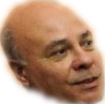
\includegraphics[height=8mm]{Sections/1-Introduccion/images/Puglesi.png}};}
}
\usepackage{tikz}
\usetikzlibrary{shapes,arrows}
%%%%%%%%%%%%%%%%%%%%%%%%%%%%%%%%%%%%%%%%%%%%%%%%%%%%%%%%%%%%%%%%%%%%%%%%%%%%%%%%
%% Front page definition

\title[{\makebox[.5\paperwidth]{PFE: Planta Móvil de Control de Nivel\hfill%
       \insertframenumber/\inserttotalframenumber}}]{Proyecto Final de Estudios}

\subtitle{Planta Móvil de Control de Nivel\\Diseño, Construcción y
Programación}
\author{\texorpdfstring{Alvaro \textbf{A}lonso\\
			Maximiliano \textbf{B}adaloni\\
			Fernando \textbf{C}ladera}
			{Alonso Badaloni Cladera}
	}

\institute{
	{\tiny Director}\\ \vspace{.10cm}
	Prof. Mg. Ing. Alfredo Ernesto Puglesi
	\\
	\vspace{.8cm}

	\begin{columns}[t]
		\begin{column}{0.145\textwidth}
		\end{column}
		\begin{column}{0.35\textwidth}
			\centering

\includegraphics[height=.75cm]{../Informe/Caratula/Logos/LogoFacu.pdf}
		\end{column}
		\begin{column}{0.35\textwidth}
			\centering

\includegraphics[height=.75cm]{../Informe/Caratula/Logos/ENIB-cmjn.png}
		\end{column}
		\begin{column}{0.145\textwidth}
		\end{column}
	\end{columns}
	%\vspace{-0.35cm}
}

\date{
  \scriptsize Facultad de Ingeniería - Universidad Nacional de Cuyo
  \\
  \vspace{.10cm}
  \today
  \ifdebug
	\quad{\color{red} DEBUG MODE!}
  \fi
}

%%%%%%%%%%%%%%%%%%%%%%%%%%%%%%%%%%%%%%%%%%%%%%%%%%%%%%%%%%%%%%%%%%%%%%%%%%%%%%%%

\begin{document}
\frame{
	\titlepage
}

%%%%%%%%%%%%%%%%%%%%%%%%%%%%%%%%%%%%%%%%%%%%%%%%%%%%%%%%%%%%%%%%%%%%%%%%%%%%%%%%

\section{Introducción}
  
\subsection*{Contexto}
% Una subsection* crea un nuevo "grupo de puntos"

\frame{
	\frametitle{Descripción del problema}

	\textbf{Objetivo}
	\vspace{0.25cm}
	\begin{center}
		“Diseñar, ensamblar y programar una planta móvil de control de 
		  nivel, utilizando sensores, controladores y actuadores 
		  industriales disponibles en el mercado”
	\end{center}
	\textbf{Es decir, algo así}...
	\begin{center}
	  \vspace{0.25cm}
	  \begin{figure}[h!]
	  \centering
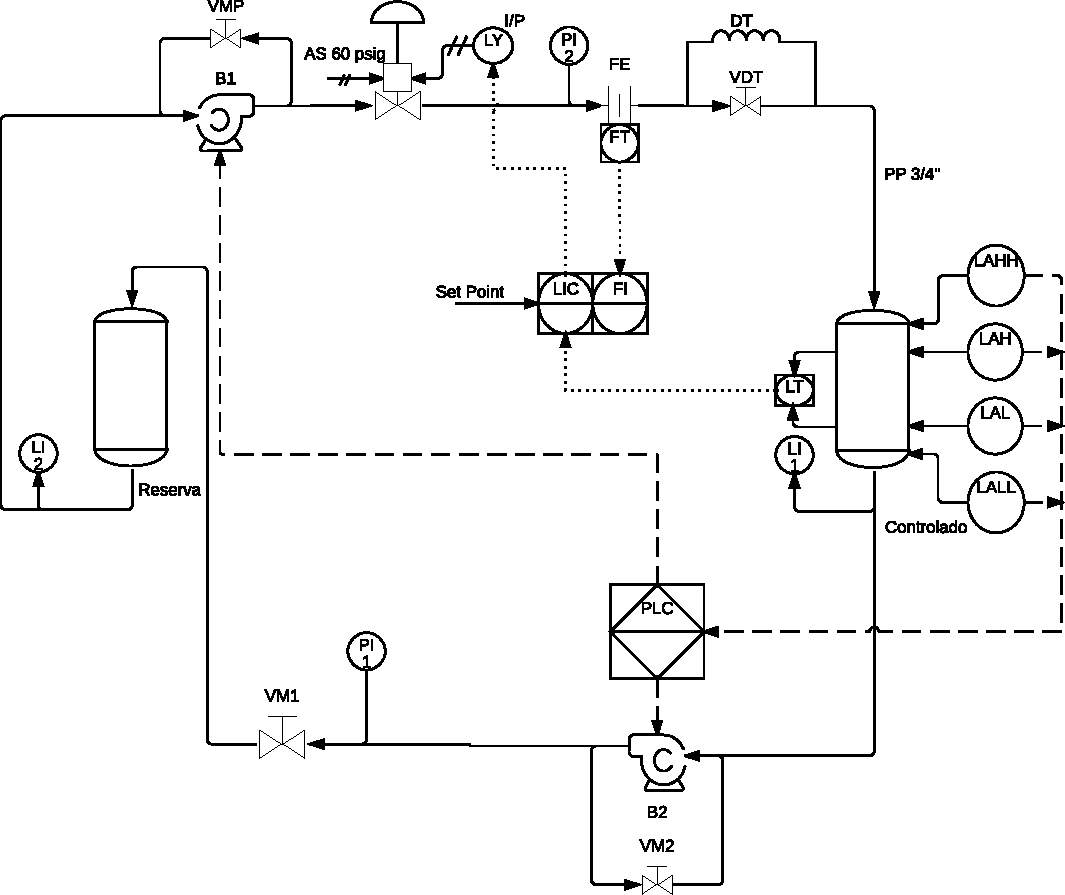
\includegraphics[width=.4\textwidth]
{Sections/1-Introduccion/images/p&id.pdf}
	  \end{figure}
	\end{center}
}

\frame{
	\frametitle{Especificaciones Vs Solución Propuesta}
	
	\textbf{Solución Propuesta}...
	\hspace{1cm}
	\textbf{Especificaciones}...
	
	
	\begin{columns}
		\begin{column}{0.4\textwidth}
		  \begin{center}
		    \begin{figure}[h!]
		      \centering
			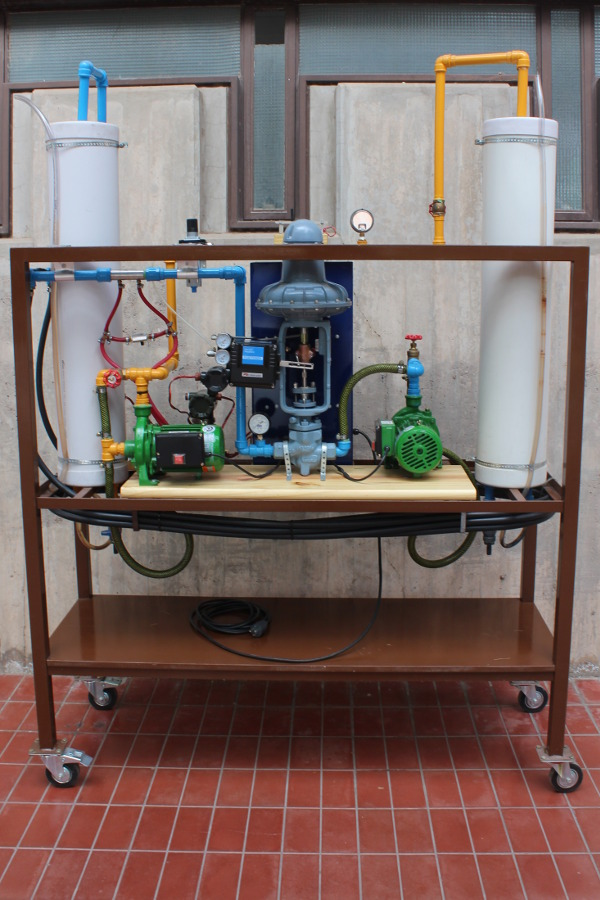
\includegraphics[width=\textwidth]
			 {Sections/1-Introduccion/images/IMG_5123.jpeg}
			\end{figure}
		   \end{center}
		\end{column}
		\begin{column}{0.5\textwidth}
		La planta debe:
			\begin{enumerate}
				\item Representar un ambiente industrial.
				\begin{itemize}
				 \item Procesos
				 \item Materiales
				\end{itemize}
				\item Cumplir un objetivo pedagógico.
				 \begin{itemize}
				  \item Verificar el funcionamiento 
del conjunto.
				  \item Documentar: Manual del usuario de la 
planta.
				 \end{itemize}
				\item Tener un costo inferior a una solución 
llave en mano.
			\end{enumerate}
		\end{column}
	\end{columns}
}

\frame{
	\frametitle{Análisis Económico}
	
	\begin{columns}
	  \centering
	 \begin{column}{0.3\textwidth}
	    \centering
	    \textbf{Cuál es el costo?}
	 \end{column}
	 
	 \begin{column}{0.3\textwidth}
	    \textbf{Plantas Similares:}
	    \begin{itemize}
	     \item Llave en mano.
	     \item Puerto de Bs.As.
	    \end{itemize}
	 \end{column}

	 \begin{column}{0.3\textwidth}
	    \begin{ukblock}
		\centering
		\textbf{16225\$} 
	    \end{ukblock}
	    \begin{itblock}
		\centering
		\textbf{\EUR{28403}}
	    \end{itblock}
	 \end{column}
	\end{columns}

	
	\vspace{-0.5cm}
	\begin{center}
%	 Las partes constitutivas de ambas plantas son elementos industriales
	 \end{center}
	\textbf{Donaciones:}
	\vspace{0.2cm}
	\begin{columns}[T]
	
	 \begin{column}{0.3\textwidth}
	    \begin{techintblock}
		\centering
		\textbf{5050\$}
	    \end{techintblock}
	    \footnotesize
	    \begin{itemize}
	     \item Electrobombas
	     \item PLC+PS+Mod. Analógico
	     \item DP Cell
	     \item Válvula de control
	    \end{itemize}
	 \end{column}
	 
	 \begin{column}{0.3\textwidth}
	    \begin{fingblock}
		\centering
		\textbf{2122\$}
	    \end{fingblock}
	    \footnotesize
	     \begin{itemize}
	      \item Estructura
	      \item Tuberías y Acc.
	      \item Material Eléctrico
	      \item Manómetros.
	     \end{itemize}
	 \end{column}

	 \begin{column}{0.3\textwidth}
	    \begin{puglesiblock}
		\centering
		\textbf{50\$}
	    \end{puglesiblock}
	    \footnotesize
	    \begin{itemize}
	     \item Placa Orificio
	    \end{itemize}

	 \end{column}

	\end{columns}
	
}

\frame{
	\frametitle{División del trabajo}
	\textbf{Idea:} ...
	\vspace{0.25cm}
	\begin{center}

		Lorem ipsum dolor sit amet, consectetur adipiscing elit.
		Donec viverra cursus pellentesque. In et mattis augue.
		Dorbi ut velit a ante ultrices ornare in id nisl.

		\vspace{0.5cm}

		Pellentesque sollicitudin bibendum leo lobortis sagittis.
		Fusce eu purus vel mauris vestibulum mattis.
	\end{center}
}

\begin{frame}
    \frametitle{Outline}
    \tableofcontents
\end{frame}

\section{Diseño y Ensamblado}
\frame{
	\frametitle{Outline}
	\tableofcontents[currentsection]
	}

\subsection*{PyID}
% Una subsection* crea un nuevo "grupo de puntos"

\frame{
	\frametitle{PyID}

	\begin{center}
		\textbf{Definición}

		\vspace{0.25cm}

		\missingfigure[figwidth=6cm]{Figura completa}
	\end{center}

	\begin{columns}
		\begin{column}{0.5\textwidth}
			\begin{itemize}
				\item {\color{newcolor} Texto en columna 1}:
				\begin{itemize}
					\item item 1
					\item item 2
				\end{itemize}
				\item {\color{newcolor} Más texto}
			\end{itemize}
		\end{column}

		\begin{column}{0.5\textwidth}
			\begin{itemize}
				\item {\color{softBlue!70!Black} Texto:}
					en otra columna
				\item {\color{softOrange!70!Black} Más texto:}
					en otra columna
			\end{itemize}

		\end{column}
	\end{columns}
}

\subsection*{Circuito hidráulico}
\frame{
	\frametitle{Cañerías y Tanques}
	\begin{columns}
		\begin{column}{0.4\textwidth}
			\begin{enumerate}
				\item Una
				\begin{itemize}
					\item \textbf{Larga}
					\item larga
				\end{itemize}
				\item Lista
			\end{enumerate}

			\begin{align*}
				\mathrm{una} \,e( \textbf{cuacion})
			\end{align*}
		\end{column}

		\begin{column}{0.6\textwidth}
			\begin{center}
				\missingfigure[figwidth=4.5cm]{}
			\end{center}

			\begin{center}
				\footnotesize
				\textbf{\textit{Cita bibliográfica}}

				[Escrita por alguien \textit{et al.} 2008]
			\end{center}
		\end{column}

	\end{columns}
}

\frame{
	\frametitle{Bombas}
	\textbf{Idea:} ...
	\vspace{0.25cm}
	\begin{center}

		Lorem ipsum dolor sit amet, consectetur adipiscing elit.
		Donec viverra cursus pellentesque. In et mattis augue.
		Dorbi ut velit a ante ultrices ornare in id nisl.

		\vspace{0.5cm}

		Pellentesque sollicitudin bibendum leo lobortis sagittis.
		Fusce eu purus vel mauris vestibulum mattis.
	\end{center}
}
\subsection*{Valv}
\frame{
	\frametitle{Valv1}
	\textbf{Idea:} ...
	\vspace{0.25cm}
	\begin{center}

		Lorem ipsum dolor sit amet, consectetur adipiscing elit.
		Donec viverra cursus pellentesque. In et mattis augue.
		Dorbi ut velit a ante ultrices ornare in id nisl.

		\vspace{0.5cm}

		Pellentesque sollicitudin bibendum leo lobortis sagittis.
		Fusce eu purus vel mauris vestibulum mattis.
	\end{center}
}
\frame{
	\frametitle{Valv2}
	\textbf{Idea:} ...
	\vspace{0.25cm}
	\begin{center}

		Lorem ipsum dolor sit amet, consectetur adipiscing elit.
		Donec viverra cursus pellentesque. In et mattis augue.
		Dorbi ut velit a ante ultrices ornare in id nisl.

		\vspace{0.5cm}

		Pellentesque sollicitudin bibendum leo lobortis sagittis.
		Fusce eu purus vel mauris vestibulum mattis.
	\end{center}
}
\frame{
	\frametitle{Valv3}
	\textbf{Idea:} ...
	\vspace{0.25cm}
	\begin{center}

		Lorem ipsum dolor sit amet, consectetur adipiscing elit.
		Donec viverra cursus pellentesque. In et mattis augue.
		Dorbi ut velit a ante ultrices ornare in id nisl.

		\vspace{0.5cm}

		Pellentesque sollicitudin bibendum leo lobortis sagittis.
		Fusce eu purus vel mauris vestibulum mattis.
	\end{center}
}


\subsection*{Instrumentación}
\frame{
	\frametitle{Placa Orificio}
	\begin{columns}
		\begin{column}{0.4\textwidth}
			\begin{enumerate}
				\item Una
				\begin{itemize}
					\item \textbf{Larga}
					\item larga
				\end{itemize}
				\item Lista
			\end{enumerate}

			\begin{align*}
				\mathrm{una} \,e( \textbf{cuacion})
			\end{align*}
		\end{column}

		\begin{column}{0.6\textwidth}
			\begin{center}
				\missingfigure[figwidth=4.5cm]{}
			\end{center}

			\begin{center}
				\footnotesize
				\textbf{\textit{Cita bibliográfica}}

				[Escrita por alguien \textit{et al.} 2008]
			\end{center}
		\end{column}

	\end{columns}
}

\frame{
	\frametitle{DP Cells}
	\textbf{Idea:} ...
	\vspace{0.25cm}
	\begin{center}

		Lorem ipsum dolor sit amet, consectetur adipiscing elit.
		Donec viverra cursus pellentesque. In et mattis augue.
		Dorbi ut velit a ante ultrices ornare in id nisl.

		\vspace{0.5cm}

		Pellentesque sollicitudin bibendum leo lobortis sagittis.
		Fusce eu purus vel mauris vestibulum mattis.
	\end{center}
}
\frame{
	\frametitle{Manómetros}
	\textbf{Idea:} ...
	\vspace{0.25cm}
	\begin{center}

		Lorem ipsum dolor sit amet, consectetur adipiscing elit.
		Donec viverra cursus pellentesque. In et mattis augue.
		Dorbi ut velit a ante ultrices ornare in id nisl.

		\vspace{0.5cm}

		Pellentesque sollicitudin bibendum leo lobortis sagittis.
		Fusce eu purus vel mauris vestibulum mattis.
	\end{center}
}

\section{Tablero y Conexionado}
\frame{
	\ifdebug
	\frametitle{Outline\hfill{\color{red} \emph{F}}}
	\else
	\frametitle{Outline}
	\fi
	\tableofcontents[currentsection]
	}

\subsection*{Generalidades}
% Una subsection* crea un nuevo "grupo de puntos"

\frame{
	\ifdebug
	\frametitle{Generalidades\hfill{\color{red} \emph{F}}}
	\else
	\frametitle{Generalidades}
	\fi

	\begin{columns}
		\begin{column}{0.55\textwidth}
		{\color{newcolor}Objetivos:}
		\begin{itemize}
		 \item \textbf{Alimentar} los elementos de la planta
		 \item \textbf{Encender} motores
		 \item \textbf{Adquisición} de variables
		 \item \textbf{Control} de la válvula
		 \item \textbf{Seguridad}
		\end{itemize}
		
		\vspace{.5cm}
		{\color{newcolor}Distinguimos:}
		\begin{itemize}
		 \item Cableado de potencia
		 \item Cableado de señal
		\end{itemize}


		\end{column}
		\begin{column}{0.45\textwidth}
			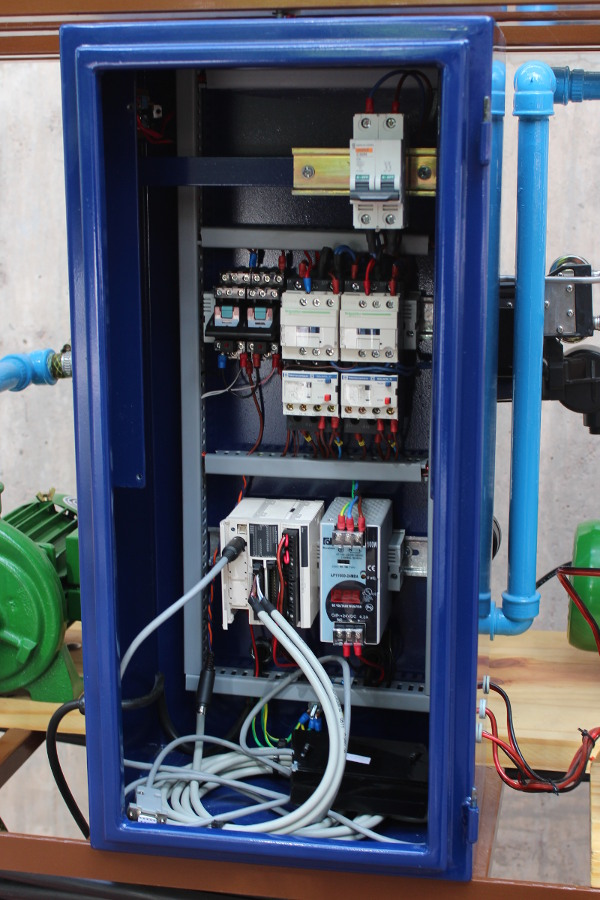
\includegraphics[width=\textwidth]
{Sections/3-Tablero/Images/IMG_5097.JPG}
		\end{column}
	\end{columns}
}

\subsection*{Cableado de potencia}
\frame{
	\ifdebug
	\frametitle{Cableado de potencia\hfill{\color{red} \emph{F}}}
	\else
	\frametitle{Cableado de potencia}
	\fi

	
	Elementos eléctricos, destinados a \textbf{alimentar} los motores de 
las bombas y los circuitos lógicos

	\vspace{-.25cm}
	\begin{columns}
	 \begin{column}{.45\textwidth}
	\begin{itemize}
	 \item \textbf{Interruptor termomagnético}
	 \item \textbf{Fuente de alimentación} $24\,V$ - $100\,W$
	 \item \textbf{Alimentación de motores}
	 \end{itemize}
	 \end{column}
	 
	 \begin{column}{.55\textwidth}
	 \begin{center}
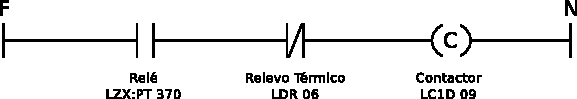
\includegraphics[width=\textwidth]{Sections/3-Tablero/Images/ladderConexion.pdf}

\vspace{.5cm}

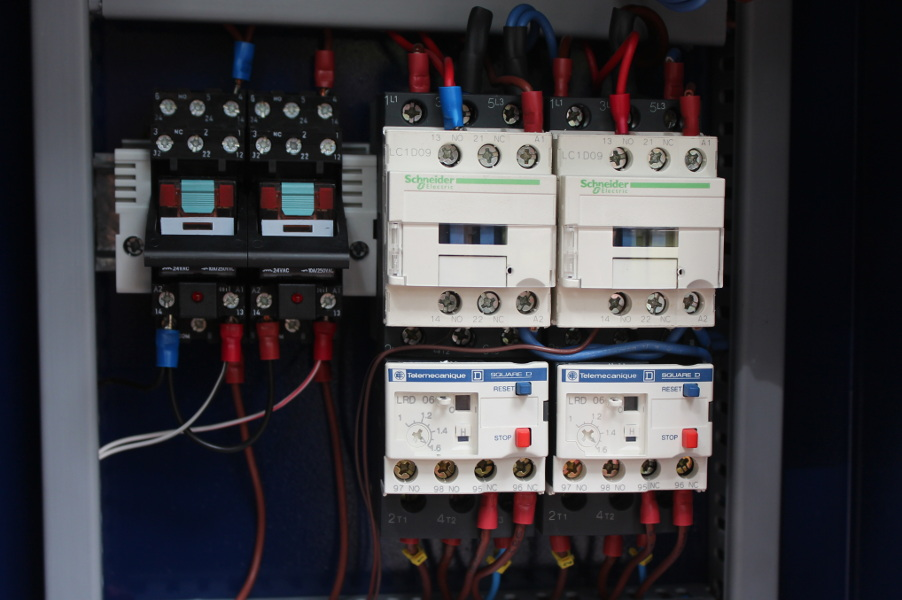
\includegraphics[width=\textwidth]{Sections/3-Tablero/Images/IMG_5093.JPG}

	\footnotesize
	Detalle alimentación de motores
	 \end{center}
	\end{column}
\end{columns}
}

\subsection*{Cableado de señal}
\frame{
	\ifdebug
	\frametitle{Cableado de señal: PLC\hfill{\color{red} \emph{F}}}
	\else
	\frametitle{Cableado de señal: PLC}
	\fi

	\textbf{Controlador Lógico Programable}
	
	\vspace{.25cm}
	\begin{columns}[t]
		\begin{column}{0.45\textwidth}
			
			\begin{itemize}
			 \item Procesador - memoria
			 \item I/O discretas
			 \begin{itemize}
			  \item Activación de motores 
			  
			  \texttt{Q0.0} - \texttt{Q0.1}
			  \item Enclavamientos 
			  
			  \texttt{I0.0} - \texttt{I0.1}
			 \end{itemize}

			 \item I/O analógicas
			 \begin{itemize}
			  \item Lectura DP Cells
			  
			  \texttt{IW0.1.0} - \texttt{IW0.1.1}
			  \item Actuador (válvula)
			 
			 \texttt{QW0.1.0}
			 \end{itemize}

			\end{itemize}

		\end{column}

		\begin{column}{0.55\textwidth}
			\begin{center}
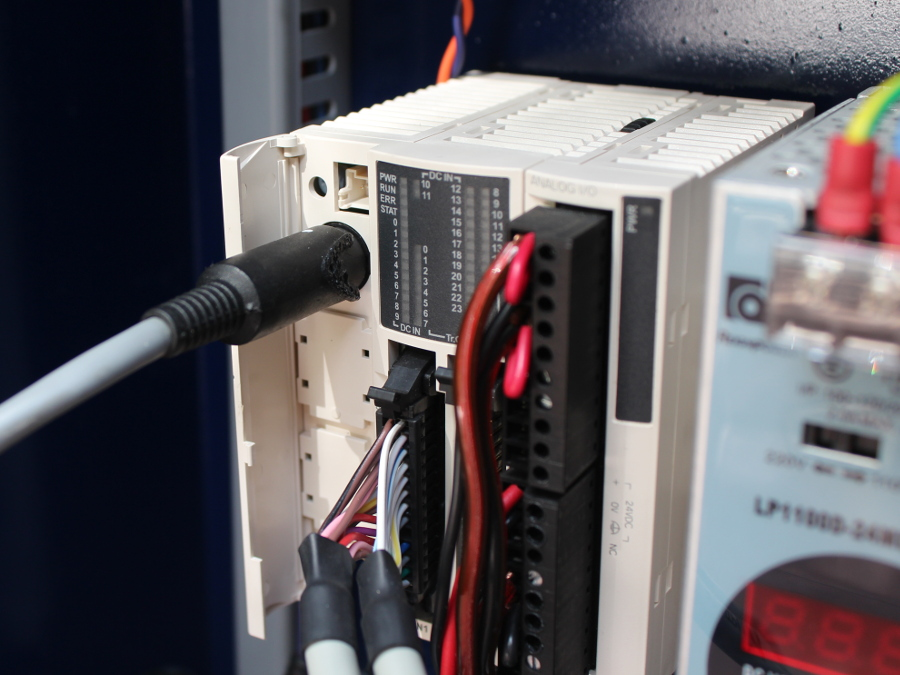
\includegraphics[width=\textwidth]{Sections/3-Tablero/Images/PLC.JPG}

			\footnotesize
			PLC Twido \texttt{40DTK}
			
			Módulo \texttt{AMM 6HT} ($4$-$20\,mA$ $12\,bits$)
			\end{center}
		\end{column}
	\end{columns}
}

\frame{
	\ifdebug
	\frametitle{Cableado de señal: Comunicación\hfill{\color{red}\emph{F}}}
	\else
	\frametitle{Cableado de señal: Comunicación}
	\fi

	
	PLC $\Rightarrow$ \texttt{RS485}
	
	Computador supervisor $\Rightarrow$ \texttt{RS232C}, \texttt{USB}
	\vspace{-.5cm}
	\begin{columns}[t]
	 \begin{column}{.5\textwidth}
	  \begin{center}
	   {\color{newcolor}Adaptador}
	  \end{center}
	  \vspace{-.25cm}
	\begin{itemize}
	 \item {\color{darkgreen1} Ventajas}

	   Inmunidad a interferencias

	 \item {\color{newcolor3} Inconvenientes}

	  Vínculo físico

	\end{itemize}
	\centering
	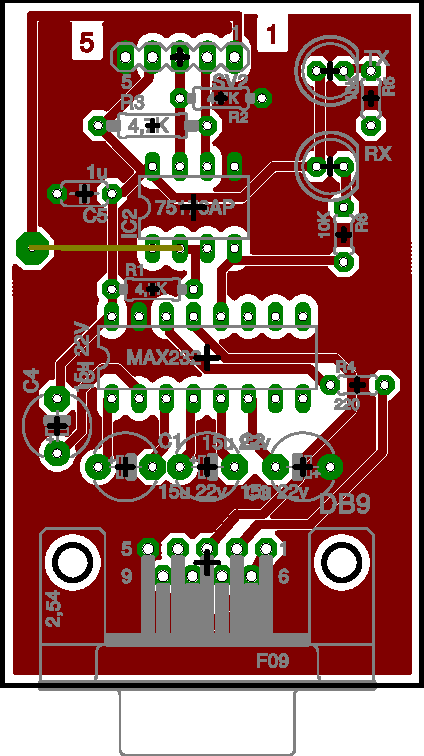
\includegraphics[height=3.85cm]
{Sections/3-Tablero/Images/Card.pdf}
	 \end{column}
	 \begin{column}{.5\textwidth}
	  \begin{center}
	  {\color{newcolor}Conexión inalámbrica}
	  \end{center}
	  \vspace{-.25cm}
	  \begin{itemize}
	 \item {\color{darkgreen1} Ventajas}

	  Móvil

	 \item {\color{newcolor3} Inconvenientes}

	  Alta latencia, timeouts


	\end{itemize}
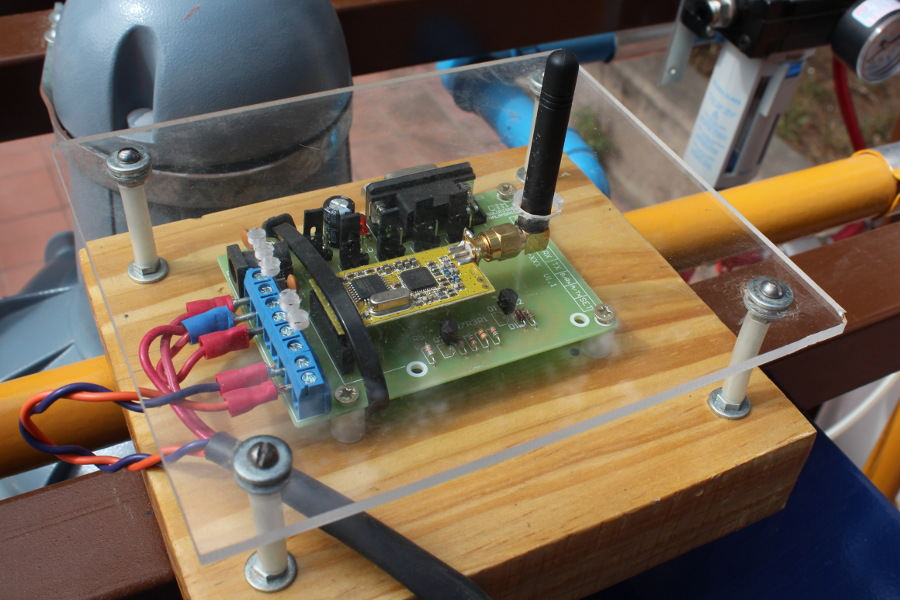
\includegraphics[width=\textwidth]
{Sections/3-Tablero/Images/IMG_5038.JPG}
	  
	 \end{column}
	\end{columns}
}
\section{PLC}
\frame{
	\frametitle{Outline}
	\tableofcontents[currentsection]
	}

\subsection*{Algoritmo}
% Una subsection* crea un nuevo "grupo de puntos"

\frame{
	\frametitle{Algoritmo}
	% Define block styles
\tikzstyle{decision} = [diamond, draw, fill=blue!20, 
    text width=4.5em, text badly centered, node distance=3cm, inner sep=0pt]
\tikzstyle{block} = [rectangle, draw, fill=blue!20, 
    text width=4em, text centered, rounded corners, minimum height=4em]
\tikzstyle{line} = [draw, -latex']

\tikzstyle{cloud} = [draw, ellipse,fill=red!20, node distance=3cm,
    minimum height=2em]
    
\begin{figure}[t]
\resizebox{0.9\textwidth}{!}{

\begin{tikzpicture}[node distance = 2cm, auto]
    % Place nodes
    \node [cloud] (init) {Tablero energizado};
    \node [block, below of=init] (run) {PLC run};
    \node [block, below of=run] (var) {Adq. Nivel y Caudal};
    \node [decision, below of=var](hhl){Nivel?};
    \node [block, below of=hhl](stop){Detener la planta};
    \node [decision, right of=hhl](hl){Nivel?};
    \node [block, below of=hl](alarm){Señal de alarma};
    \node [decision, right of=hl](set){Parám.?};
    \node [block, below of=set](param){Seteo de parámetros};
    \node [decision, right of=set](manual){Manual?};
    \node [block, below of=manual](control){Control manual};
    \node [block, right of=manual](on){Motores ON};
    \node [block, right of=on](state){Estado};
    \node [, below left of=stop](null){};
    %\node (null){};
%     % Draw edges
    \path [line,dashed] (init) -- (run);
    \path [line] (run) -- (var);
    \path [line] (var) -- (hhl);
    \path [line] (hhl) -- node {si} (stop) ;
    \path [line] (stop) |- (null);
    \path [line] (null) |- (run);%--++  (-3,0) |- (run);
    \path [line] (hhl) -- (hl);
    \path [line] (hl) -- node {si} (alarm);
    \path [line] (hl) -- (set);
    \path [line] (set) -- node {si} (param);
    \path [line] (set) -- (manual);
    \path [line] (manual) -- node {si} (control);
    \path [line] (manual) -- (on);
    \path [line] (on) -- (state);
    \path [line] (state) |- (null);
    \path [line] (alarm) |- (null);
    \path [line] (param) |- (null);
    \path [line] (control) |- (null);

\end{tikzpicture}
 }
\end{figure}


}

\frame{
	\frametitle{Programación}
	\textbf{Lenguaje de Programación}
	\begin{itemize}
	 \item {\color{newcolor} Ladder:} Lenguaje gráfico de programación.
	 \item {\color{newcolor} Palabras de Memorias}
	\end{itemize}
	
\begin{table}[!t]
\tiny
\renewcommand{\arraystretch}{1.3}
\centering
\begin{tabular}{c||c||c}
\hline
\bfseries Tipo & \bfseries Word  & \bfseries Descripción\\
\hline \hline
Lect & MW2  & Lectura DP cell nivel \\
Lect & MW3  & Lectura DP cell caudal\\
Lect & MW4  & Valor Kp\\
Lect & MW5  & Valor Ti\\
Lect & MW6  & Valor Td\\
Lect & MW7  & Valor de lectura del SP \\
Lect & MW8  & Valor de lectura de la válvula \\
\hline
Esc & MW9 & Valor de escritura de la válvula (manual)\\
Esc & MW10  & Valor de escritura del SP \\
Esc & MW11  & Valor de escritura Kp \\
Esc & MW12  & Valor de escritura Ti \\
Esc & MW13  & Valor de escritura Td \\
\hline
\end{tabular}
\end{table}

}
\frame{
	\frametitle{Programación}
	\begin{table}[!t]
	\tiny
\renewcommand{\arraystretch}{1.3}
\centering
\begin{tabular}{c||c||c||c}
\hline
\bfseries Tipo & \bfseries Word & \bfseries Bit & \bfseries Descripción\\
\hline \hline
Lect & MW0 & X0 & Señal Run PLC\\
Lect & & X1 & Alarma HHL\\
Lect & & X2& Alarma LLL\\
Lect & & X3& Alarma HL\\
Lect & & X4& Alarma LL\\
Lect & & X5& Error en motores\\
Lect & & X6& Motor 1 encendido\\
Lect & & X7& Motor 2 encendido\\
Lect & & X8& Modo manual activado\\
Lect & & X9& Modo automático activado y funcionando\\
Lect & & X10& Planta funcionando sin errores\\
\hline
Esc & MW1 & X0& Switch Encender(1)/Apagar(0)\\
Esc & & X1& Manual(1)/Automático(0)\\
Esc & & X2& Cambiar parámetros PID\\
Esc & & X3& Cambiar Set Point\\
Esc & & X4& Manual(0)/Default(1)\\
Esc & & X5& Encender M1 (manual)\\
Esc & & X6& Encender M2 (manual)\\
Esc & & X7& Limpiar errores\\
Esc & & X8& Parada de emergencia\\
Esc & & X9& Limpiar señal de parada de emergencia\\
\hline
\end{tabular}

\end{table}

}


\frame{
	\frametitle{Controlador PID}
	\textbf{Acción del controlador:}
	%{\color{newcolor} Acción de controlador}
	\begin{itemize}
	  \item Proporcional al error.
	  \item Proporcional a la integral del error respecto del tiempo.
	  \item Proporcional a la derivada del error respecto del tiempo.
	 \end{itemize}
	 \vspace{0.25cm}
	\begin{columns}
		\begin{column}{0.5\textwidth}
		{\color{newcolor} Método de Ziegler–Nichols}
			\begin{center}
				\vspace{0.25cm}
				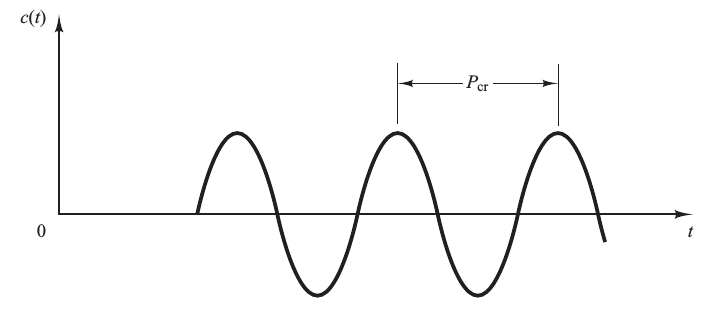
\includegraphics[width=5.4cm]{Sections/4-PLC/Images/segundometodo.png}
			\end{center}
		\end{column}

		\begin{column}{0.5\textwidth}
			\begin{table}[!t]
			\renewcommand{\arraystretch}{1.3}
			\centering
			\begin{tabular}{c||c||c}
			\hline
			\bfseries Kp  & \bfseries Ti & \bfseries Td\\
			\hline \hline
			 $0.6 \,Kp_{cr}  $ & $ 0.5 \, P_{cr}$ & $0.125 \, P_{cr} $\\
			\hline
			\end{tabular}
			\end{table}
		\end{column}

	\end{columns}
}

\frame{
	\frametitle{PID tunning}
	\textbf{Ganancias del controlador}
	%{\color{newcolor} Ganancias del controlador}
	\begin{columns}
		\begin{column}{0.6\textwidth}
			\begin{center}
			\vspace{0.25cm}
				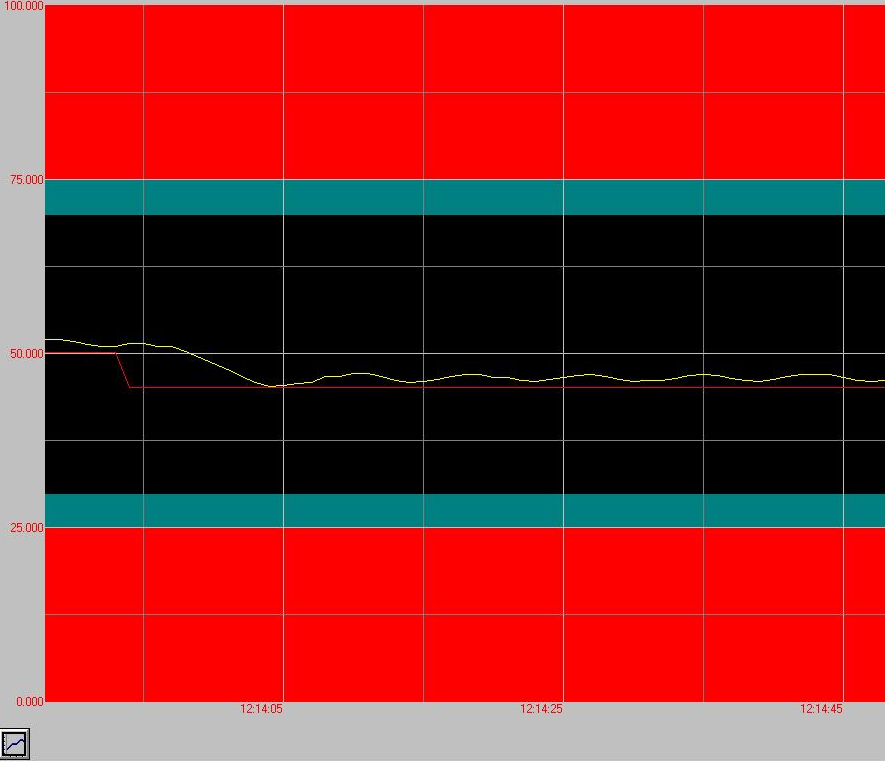
\includegraphics[width=5.5cm]{Sections/4-PLC/Images/oscperm.png}
			\end{center}
		\end{column}
		\begin{column}{0.4\textwidth}
			\begin{itemize}

			 \item {\color{newcolor2} Sin tiempo muerto:}
			    \begin{itemize}
			      \item $K_p $: $36$
			      \item $T_i $: $4$
			      \item $T_d $: $1$ 
			    \end{itemize}
			\end{itemize}
		\end{column}

	\end{columns}
}

\frame{
	\frametitle{PID tunning}
	\textbf{Ganancias del controlador}
	%{\color{newcolor} Ganancias del controlador}
	\begin{columns}
		\begin{column}{0.6\textwidth}
			\begin{center}
			\vspace{0.25cm}
				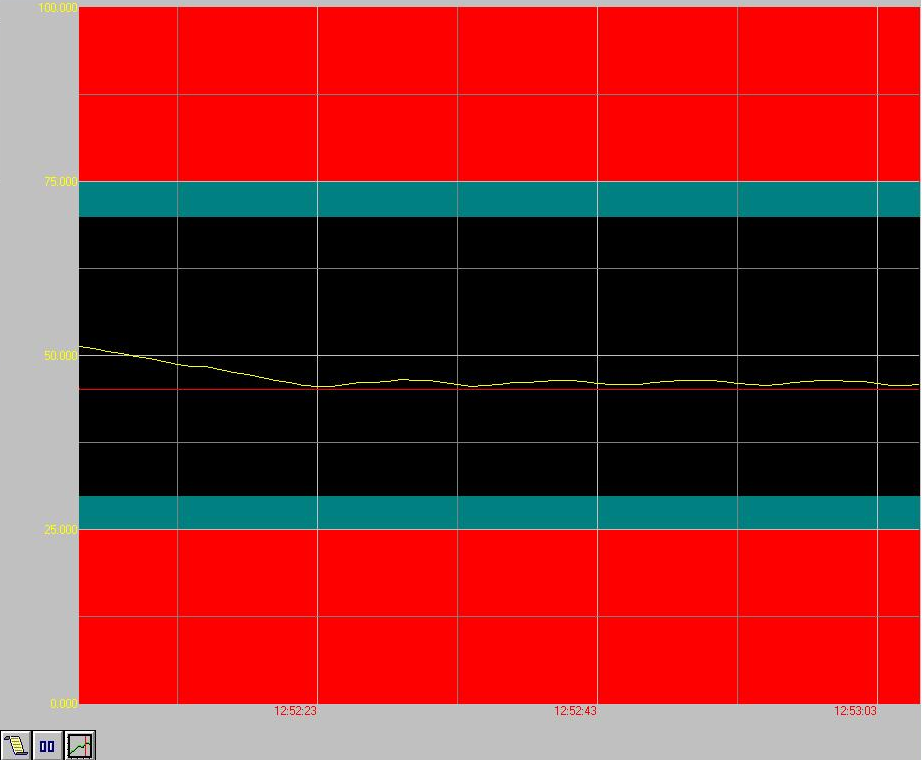
\includegraphics[width=5.5cm]{Sections/4-PLC/Images/oscpermtd.png}
			\end{center}
		\end{column}
		\begin{column}{0.4\textwidth}
			\begin{itemize}
			 \item {\color{newcolor2} Con tiempo muerto:}
			    \begin{itemize}
			      \item $K_p $: $72$
			      \item $T_i $: $5$
			      \item $T_d $: $1.25$ 
			    \end{itemize}
			\end{itemize}
		\end{column}

	\end{columns}
}

\section{SCADA}
\frame{
	\ifdebug
	\frametitle{Outline\hfill{\color{red} \emph{A}}}
	\else
	\frametitle{Outline}
	\fi
	\tableofcontents[currentsection]
	}

\subsection*{Intro Scada}

\frame{
	\ifdebug
	\frametitle{Introducción SCADA\hfill{\color{red} \emph{A}}}
	\else
	\frametitle{Introducción SCADA}
	\fi
	\textbf{PLC:} realiza automáticamente las tareas de control 
	    pre-programado sobre un proceso.
	   
	\textbf{Problema:} no presenta una manera amigable de
	\begin{columns}
	 \begin{column}{0.3\textwidth}
	 \begin{itemize}
	   \item Supervisar
	   \item Adaptar
	 \end{itemize}
	 \end{column}
	 \begin{column}{0.7\textwidth}
	  El comportamiento del sistema
	 \end{column}
	\end{columns}
	
	\begin{columns}
	\begin{column}{0.5\textwidth}
	  \textbf{Solución}:\\
	  \textbf{SCADA}: Supervisory Control And Data Adquisition
	 \end{column}
	 \begin{column}{0.5\textwidth}
	  \begin{figure}[ht!]
	    \centering
	    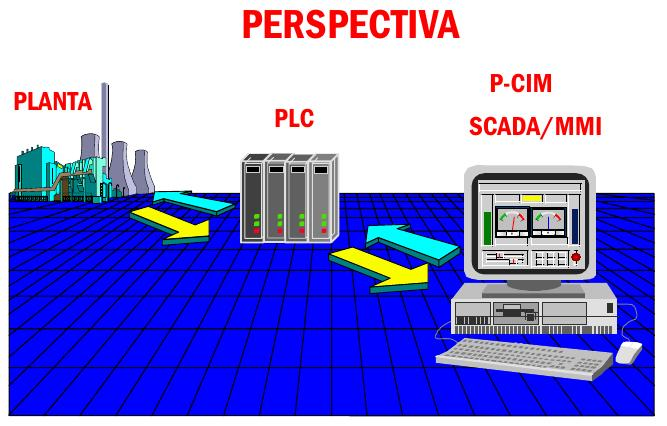
\includegraphics[width=\textwidth]
	    {../Informe/Cap5-SCADA/images/perspectiva.jpeg}
	\end{figure}
	 \end{column}
	\end{columns}
}

\subsection*{Estructura PCIM}
\frame{
	\ifdebug
	\frametitle{P-CIM - AFCON\hfill{\color{red} \emph{A}}}
	\else
	\frametitle{P-CIM - AFCON}
	\fi
	\begin{columns}[T]
	  \begin{column}{0.3\textwidth}
	    \begin{figure}
	      \centering
	      
\includegraphics[width=\textwidth]
	      {Sections/5-Scada/images/afcon.pdf}
	    \end{figure}
	      \footnotesize
	      Entorno de desarrollo y ejecución de aplicaciones SCADA.
	  \end{column}	 
	  \begin{column}{0.6\textwidth}
	    Su estructura se compone de 3 capas:
	    \begin{itemize}
	     \item Comunicación
	     \item Procesamiento de Datos
	     \item Aplicaciones
	    \end{itemize}
	  \begin{figure}[ht!]
	  \centering
		  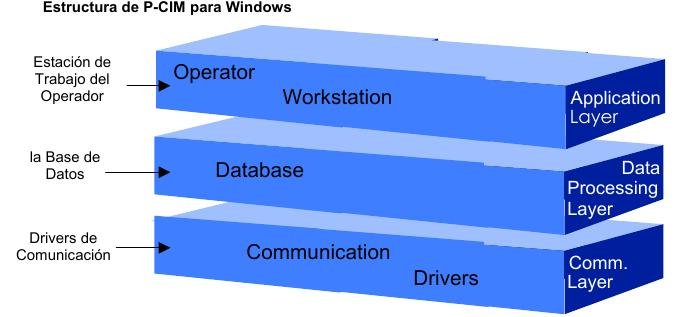
\includegraphics[width=\textwidth]
		  {../Informe/Cap5-SCADA/images/estructura.jpeg}
	  \end{figure}
	  \end{column}

	\end{columns}
}

\frame{
	\ifdebug
	\frametitle{Capa de comunicación\hfill{\color{red} \emph{A}}}
	\else
	\frametitle{Capa de comunicación}
	\fi
	\begin{columns}
	 \begin{column}{0.4\textwidth}
	    \textbf{Modbus}:\begin{itemize}
	                       \item Protocolo de facto en la industria
	                       \item Gran disponibilidad
	                       \item Libre desde 2004
	                      \end{itemize}

	  \end{column}
	  \begin{column}{0.6\textwidth}
	    \begin{figure}
	     
\includegraphics[width=\textwidth]
	      {Sections/5-Scada/images/modbus_logo.png}
	    \end{figure}
	  \end{column}
	\end{columns}

	\vspace{1cm}
	Para la implementación de la capa de comunicación en P-CIM:
	\begin{columns}[T]
	  \begin{column}{0.3\textwidth}
	    \textbf{Instalación}
	    \begin{figure}
	     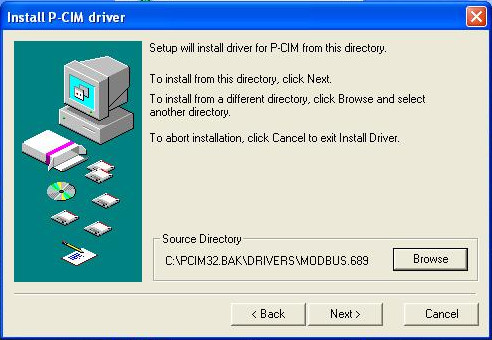
\includegraphics[width=\textwidth]
	      {../Informe/Cap5-SCADA/images/installDriver.jpeg}
	    \end{figure}
	  \end{column}
	  \begin{column}{0.3\textwidth}
	   \textbf{Configuración}
	   \begin{figure}
	    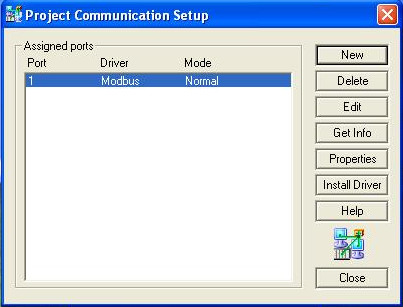
\includegraphics[width=\textwidth]
	      {../Informe/Cap5-SCADA/images/commSetup.jpeg}
	   \end{figure}
	  \end{column}
	  \begin{column}{0.3\textwidth}
	   \textbf{Obtener Información}
	  \begin{figure}
	   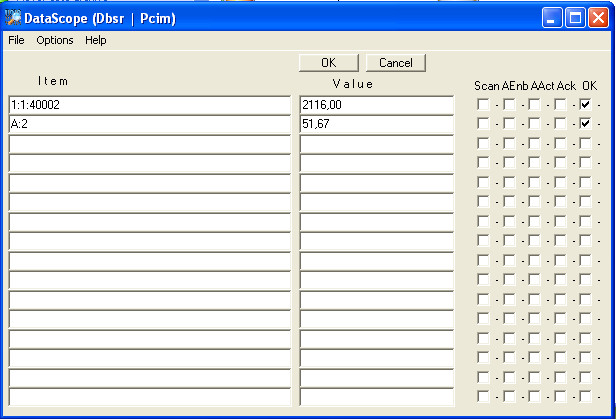
\includegraphics[width=0.8\textwidth]
	    {../Informe/Cap5-SCADA/images/dataScope.jpeg}
	  \end{figure}
	 \end{column}
	\end{columns}
}

\frame{
	\ifdebug
	\frametitle{Capa de procesamiento\hfill{\color{red} \emph{A}}}
	\else
	\frametitle{Capa de procesamiento}
	\fi
	\textbf{Base de Datos}: recupera, almacena y procesa la
información de tiempo real que recibe desde la capa de comunicación
	\begin{figure*}[!ht]
  \centering 
  \resizebox{\textwidth}{!}{
  
  \begin{tikzpicture}[shorten >=1pt,->,draw=black!50]
    \tikzstyle{every pin edge}=[<-,shorten <=1pt, ultra thick]
    \tikzstyle{neuron}=[rectangle,fill=black!25,minimum size=17pt,inner 
sep=4pt, rounded corners]
    \tikzstyle{annot} = [text width=7em, text centered]

    \tikzstyle{plc neuron}=[neuron, fill=green!50];
    \tikzstyle{modbus neuron}=[neuron, fill=red!50, node 
    distance=0.4*5cm];
    \tikzstyle{aio neuron}=[neuron, fill=blue!50, node 
    distance=0.75*5cm];
    \tikzstyle{calc neuron}=[neuron, fill=yellow!50, node 
    distance=0.75*5cm];
    \tikzstyle{emul neuron}=[neuron, fill=orange!50, node 
    distance=0.85*5cm];
    \tikzstyle{emula neuron}=[neuron, fill=green!50, node 
    distance=0.6*5cm];

    % Draw the plc layer nodes
     \node[plc neuron, pin=left:Entradas/Salidas] (mw0) at (0,0) 
{\texttt{MW0}};
     \node[plc neuron, pin=left:Nivel] (mw1) at (0,-1) 
{\texttt{MW1}};
     \node[plc neuron, pin=left: Consigna Leer] (mw2) at (0,-2) 
{\texttt{MW2}};
     \node[plc neuron, pin=left: Consigna Escribir] (mw10) at (0,-3) 
{\texttt{MW10}};
     \node[plc neuron, pin=left: Caudal] (mw3) at (0,-4) 
{\texttt{MW3}};
      \node[plc neuron, pin=left: Kp Leer] (mw4) at (0,-5) 
 {\texttt{MW4}};
      \node[plc neuron, pin=left: Kp Escribir] (mw11) at (0,-6) 
 {\texttt{MW11}};
      \node[plc neuron, pin=left: Ti Leer] (mw5) at (0,-7) 
 {\texttt{MW5}};
      \node[plc neuron, pin=left: Ti Escribir] (mw12) at (0,-8) 
 {\texttt{MW12}};
      \node[plc neuron, pin=left: Td Leer] (mw6) at (0,-9) 
 {\texttt{MW6}};
      \node[plc neuron, pin=left: Td Escribir] (mw13) at (0,-10) 
 {\texttt{MW13}};
      \node[plc neuron, pin=left: Valvula Leer] (mw7) at (0,-11) 
 {\texttt{MW7}};
      \node[plc neuron, pin=left: Valvula Escrbir] (mw15) at (0,-12) 
 {\texttt{MW15}};
      \node[plc neuron, pin=left: Motores] (mw8) at (0,-13) 
 {\texttt{MW8}};

    %Draw Modbus layer nodes
    \node[modbus neuron, right of=mw0] (40001)  {\texttt{1:1:40001}};
    \node[modbus neuron, right of=mw1] (40002)  {\texttt{1:1:40002}};
    \node[modbus neuron, right of=mw2] (40003)  {\texttt{1:1:40003}};
    \node[modbus neuron, right of=mw3] (40004)  {\texttt{1:1:40004}};
    \node[modbus neuron, right of=mw4] (40005)  {\texttt{1:1:40005}};
    \node[modbus neuron, right of=mw5] (40006)  {\texttt{1:1:40006}};
    \node[modbus neuron, right of=mw6] (40007)  {\texttt{1:1:40007}};
    \node[modbus neuron, right of=mw7] (40008)  {\texttt{1:1:40008}};
    \node[modbus neuron, right of=mw8] (40009)  {\texttt{1:1:40009}};
    \node[modbus neuron, right of=mw10] (40011)  {\texttt{1:1:40011}};
    \node[modbus neuron, right of=mw11] (40012)  {\texttt{1:1:40012}};
    \node[modbus neuron, right of=mw12] (40013)  {\texttt{1:1:40013}};
    \node[modbus neuron, right of=mw13] (40014)  {\texttt{1:1:40014}};
    \node[modbus neuron, right of=mw15] (40016)  {\texttt{1:1:40016}};
     
    %Draw Analog Input Output layer nodes
    \node[aio neuron, right of=40001] (io)  {\texttt{ENTRADAS\_DISCRETAS}};
    \node[aio neuron, right of=40002] (niv)  {\texttt{NIVEL\_TANQUE}};
    \node[aio neuron, right of=40003] (spr)  {\texttt{SP\_READ}};
    \node[aio neuron, right of=40004] (caudal)  {\texttt{CAUDAL}};
    \node[aio neuron, right of=40005] (kpr)  {\texttt{KP\_READ}};
    \node[aio neuron, right of=40006] (tir)  {\texttt{TI\_READ}};
    \node[aio neuron, right of=40007] (tdr)  {\texttt{TD\_READ}};
    \node[aio neuron, right of=40008] (vr)  {\texttt{VALVE\_READ}};
    \node[aio neuron, right of=40009] (md)  {\texttt{MOTOR\_DIGITAL}};
    \node[aio neuron, right of=40011] (spw)  {\texttt{SP\_WRITE}};
    \node[aio neuron, right of=40012] (kpw)  {\texttt{KP\_WRITE}};
    \node[aio neuron, right of=40013] (tiw)  {\texttt{TI\_WRITE}};
    \node[aio neuron, right of=40014] (tdw) {\texttt{TD\_WRITE}};
    \node[aio neuron, right of=40016] (vw)  {\texttt{VALVE\_WRITE}};

    %Draw Calculation
    \node[calc neuron, right of=niv] (cniv) {\texttt{CALC\_NIVEL}};
    \node[calc neuron, right of=spr] (cspr) {\texttt{CALC\_SP\_READ}};
    \node[calc neuron, right of=spw] (cspw) {\texttt{CALC\_SP\_WRITE}};
    \node[calc neuron, right of=caudal] (ccaudal) {\texttt{CALC\_CAUDAL}};
    \node[calc neuron, right of=vr] (cvr) {\texttt{CALC\_VALVE\_READ}};
    \node[calc neuron, right of=vw] (cvw) {\texttt{CALC\_VALVE\_WRITE}};
    
    %Draw ResultCalculation
    \node[emul neuron, right of=cniv] (eniv) {\texttt{EMUL\_NIVEL}};
    \node[emul neuron, right of=cspr] (espr) {\texttt{EMUL\_SP\_READ}};
    \node[emul neuron, right of=cspw] (espw) {\texttt{EMUL\_SP\_WRITE}};
    \node[emul neuron, right of=ccaudal] (ecaudal) {\texttt{EMUL\_CAUDAL}};
    \node[emul neuron, right of=cvr] (evr) {\texttt{EMUL\_VALVE\_READ}};
    \node[emul neuron, right of=cvw] (evw) {\texttt{EMUL\_VALVE\_WRITE}};
    
    %Draw Emulation
    \node[emul neuron] (eio) at (2.75*5cm,0 cm) 
{\texttt{EMUL\_ENT\_DISCRETAS}};
    \node[emul neuron] (ekpr) at (2.75*5cm,-5 cm) 
{\texttt{EMUL\_KP\_READ}};
    \node[emul neuron] (etir) at (2.75*5cm,-7 cm) 
{\texttt{EMUL\_TI\_READ}};
    \node[emul neuron] (etdr) at (2.75*5cm,-9 cm) 
{\texttt{EMUL\_TD\_READ}};
    \node[emul neuron] (emd) at (2.75*5cm,-13 cm) 
{\texttt{EMUL\_MOT\_DIGITAL}};
    \node[emul neuron] (ekpw) at (2.75*5cm,-6 
cm){\texttt{EMUL\_KP\_WRITE}};
    \node[emul neuron] (etiw) at (2.75*5cm,-8 cm) 
{\texttt{EMUL\_TI\_WRITE}};
    \node[emul neuron] (etdw) at (2.75*5cm,-10 cm) 
{\texttt{EMUL\_TD\_WRITE}};

    %Draw internal variables
   \node[emula neuron, pin=right:Entradas/Salidas,right of=eio] (a1) 
  {\texttt{A:1}};
  \node[emula neuron, pin=right:Entradas/Salidas,right of=eniv] (a2) 
  {\texttt{A:2}};
  \node[emula neuron, pin=right:Entradas/Salidas,right of=espr] (a3) 
  {\texttt{A:3}};
  \node[emula neuron, pin=right:Entradas/Salidas,right of=espw] (a11) 
  {\texttt{A:11}};
  \node[emula neuron, pin=right:Entradas/Salidas,right of=ecaudal] (a4) 
  {\texttt{A:4}};
  \node[emula neuron, pin=right:Entradas/Salidas,right of=ekpr] (a5) 
  {\texttt{A:5}};
  \node[emula neuron, pin=right:Entradas/Salidas,right of=ekpw] (a12) 
  {\texttt{A:12}};
  \node[emula neuron, pin=right:Entradas/Salidas,right of=etir] (a6) 
  {\texttt{A:6}};
  \node[emula neuron, pin=right:Entradas/Salidas,right of=etiw] (a13) 
  {\texttt{A:13}};
  \node[emula neuron, pin=right:Entradas/Salidas,right of=etdr] (a7) 
  {\texttt{A:7}};
  \node[emula neuron, pin=right:Entradas/Salidas,right of=etdw] (a14) 
  {\texttt{A:14}};
  \node[emula neuron, pin=right:Entradas/Salidas,right of=evr] (a8) 
  {\texttt{A:8}};
  \node[emula neuron, pin=right:Entradas/Salidas,right of=evw] (a16) 
  {\texttt{A:16}};
  \node[emula neuron, pin=right:Entradas/Salidas,right of=emd] (a9) 
  {\texttt{A:9}};

   
  % Connect every node 
  %PLC -> MODBUS
  \path (mw0) edge[<->,ultra thick] (40001); 
  \path (mw1) edge[ultra thick] (40002); 
  \path (mw2) edge[ultra thick] (40003);
  \path (mw3) edge[ultra thick] (40004); 
  \path (mw4) edge[ultra thick] (40005); 
  \path (mw5) edge[ultra thick] (40006); 
  \path (mw6) edge[ultra thick] (40007); 
  \path (mw7) edge[ultra thick] (40008); 
  \path (mw8) edge[<->,ultra thick] (40009);
  \path (mw10) edge[ultra thick] (40011); 
  \path (mw11) edge[ultra thick] (40012); 
  \path (mw12) edge[ultra thick] (40013);
  \path (mw13) edge[ultra thick] (40014); 
  \path (mw15) edge[ultra thick] (40016); 

  %MODBUS -> Analog IO
  \path (40001) edge[<->,ultra thick] (io); 
  \path (40002) edge[ultra thick] (niv); 
  \path (40003) edge[ultra thick] (spr);
  \path (40004) edge[ultra thick] (caudal);
  \path (40005) edge[ultra thick] (kpr);
  \path (40006) edge[ultra thick] (tir);
  \path (40007) edge[ultra thick] (tdr); 
  \path (40008) edge[ultra thick] (vr);
  \path (40009) edge[<->,ultra thick] (md); 
  \path (spw) edge[ultra thick] (40011); 
  \path (kpw) edge[ultra thick] (40012);
  \path (tiw) edge[ultra thick] (40013); 
  \path (tdw) edge[ultra thick] (40014);
  \path (vw) edge[ultra thick] (40016); 

  %Analog -> Calc
  \path (niv) edge[ultra thick] (cniv);
  \path (spr) edge[ultra thick] (cspr);
  \path (cspw) edge[ultra thick] (spw);
  \path (caudal) edge[ultra thick] (ccaudal);
  \path (vr) edge[ultra thick] (cvr);
  \path (cvw) edge[ultra thick] (vw);

  %Calc -> Emulation
  \path (cniv) edge[ultra thick] (eniv);
  \path (cspr) edge[ultra thick] (espr);
  \path (espw) edge[ultra thick] (cspw);
  \path (ccaudal) edge[ultra thick] (ecaudal);
  \path (cvr) edge[ultra thick] (evr);
  \path (evw) edge[ultra thick] (cvw); 
  
  %Analog IO -> Emulation
  \path (io) edge[<->,ultra thick] (eio);
  \path (kpr) edge[ultra thick] (ekpr);
  \path (ekpw) edge[ultra thick] (kpw);
  \path (tir) edge[ultra thick] (etir);
  \path (etiw) edge[ultra thick] (tiw);
  \path (tdr) edge[ultra thick] (etdr);
  \path (etdw) edge[ultra thick] (tdw);
  \path (md) edge[<->,ultra thick] (emd);

  %Emulation -> Address
  \path (eio) edge[<->,ultra thick] (a1);
  \path (eniv) edge[ultra thick] (a2);
  \path (espr) edge[ultra thick] (a3);
  \path  (a11) edge[ultra thick] (espw);
  \path (ecaudal) edge[ultra thick] (a4);
  \path (ekpr) edge[ultra thick] (a5);
  \path  (a12) edge[ultra thick] (ekpw);
  \path (etir) edge[ultra thick] (a6);
  \path  (a13) edge[ultra thick] (etiw);
  \path (etdr) edge[ultra thick] (a7);
  \path (a14) edge[ultra thick] (etdw);
  \path (evr) edge[ultra thick] (a8);
  \path (a16) edge[ultra thick] (evw);
  \path (emd) edge[<->,ultra thick] (a9);
  

 
  % Annotate the layers
  \node[annot,above of=mw0, node distance=1cm] (plc) {PLC};
  \node[annot,above of=40001, node distance=1cm] (modbus) {MODBUS Address};
  \node[annot,above of=io, node distance=1cm] (aio) {Analog Input Ouput};
  \node[annot,right of=aio, node distance=0.75*5cm] (calc) {Calculation};
  \node[annot,above of=eio, node distance=1cm] (emul) {Emulation};
  \node[annot,above of=a1, node distance=1cm] (emula) {Emulation Address};

\end{tikzpicture}
  }
    \caption{Conexion de bloques de la Base de Datos}
    \label{fig:bloqDB}
\end{figure*}
}

\frame{
	\ifdebug
	\frametitle{Capa de aplicación\hfill{\color{red} \emph{A}}}
	\else
	\frametitle{Capa de aplicación}
	\fi
	Última capa del SCADA, antes de que la información llegue al operario

	\vspace{.5cm}
	\begin{columns}[t]
	\begin{column}{0.35\textwidth}
	\textbf{Requerimientos:}
	\begin{itemize}
	\item Reducir la complejidad de la supervisión del sistema
	\item Actuar de manera remota sobre la planta y su controlador
	\end{itemize}
	\end{column}
	\begin{column}{0.65\textwidth}
	\textbf{Diseño:}
	\begin{figure}[!ht]
	\centering
	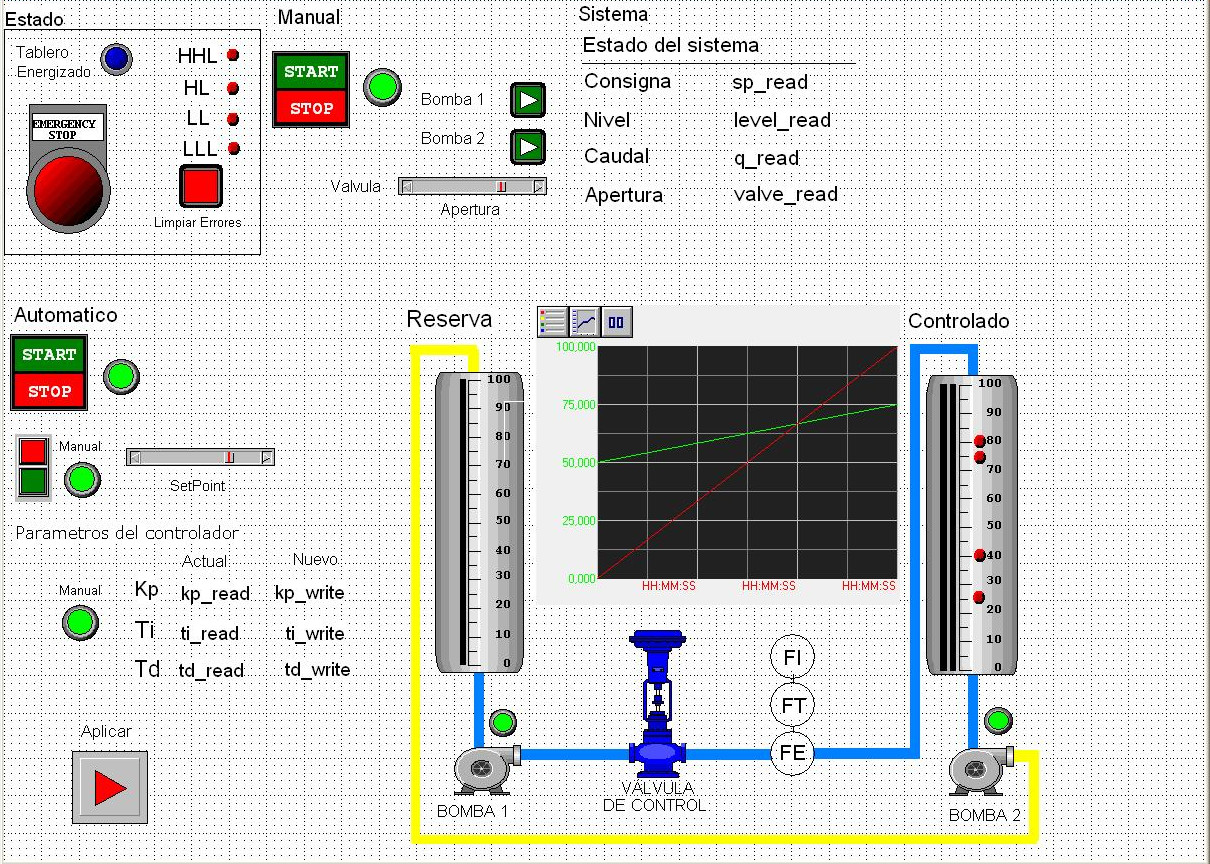
\includegraphics[width=\textwidth]
	{../Informe/Cap5-SCADA/images/hmiScada.jpeg}
	\end{figure}

	\end{column}

	\end{columns}
}

% \frame{
% 	\frametitle{Slide de gracia}
% 	\begin{columns}
% 		\begin{column}{0.4\textwidth}
% 			\begin{enumerate}
% 				\item Una
% 				\begin{itemize}
% 					\item \textbf{Larga}
% 					\item larga
% 				\end{itemize}
% 				\item Lista
% 			\end{enumerate}
% 
% 			\begin{align*}
% 				\mathrm{una} \,e( \textbf{cuacion})
% 			\end{align*}
% 		\end{column}
% 
% 		\begin{column}{0.6\textwidth}
% 			\begin{center}
% 				\missingfigure[figwidth=4.5cm]{}
% 			\end{center}
% 
% 			\begin{center}
% 				\footnotesize
% 				\textbf{\textit{Cita bibliográfica}}
% 
% 				[Escrita por alguien \textit{et al.} 2008]
% 			\end{center}
% 		\end{column}
% 
% 	\end{columns}
% }
\section{Conclusiones - Referencias}
\frame{
	\frametitle{Outline}
	\tableofcontents[currentsection]
}

\subsection*{Conclusiones}

\frame{
	\frametitle{Conclusiones y Perspectivas}
	\textbf{Conclusiones}
	\begin{itemize}
		\item {\color{newcolor} Objetivos cumplidos}
		\item {\color{newcolor} Planta pedagógica funcionando}
		\item {\color{newcolor} Más cerca de ser ingenieros}
	\end{itemize}

	\vspace{0.5cm}
	\textbf{Perspectivas}
	\begin{itemize}
		\item {\color{newcolor} Esquema de control avanzado tipo 
maestro-esclavo}
		\item {\color{newcolor} Ziegler–Nichols a lazo abierto}
	\end{itemize}
}

\subsection*{Referencias}
\frame{

	\textbf{Referencias}
	\footnotesize
	\begin{itemize}

		\item
		A. E. Puglesi, M. S. Bernasconi, E. B. Castiglione y otros,
		``Apuntes de Instrumentación y Control Automático''.
		Facultad de Ingeniería,
		UNCuyo,
		2014.

		\item
		J. B. Franzini y E. J. Finnemore,
		\textit{Mecánica de Fluidos con aplicaciones en Ingeniería}.
		McGraw-Hill,
		1999.

		\item
		I. J. Gálvez,
		``Apuntes de Mecánica de Fluidos''.
		Facultad de Ingeniería,
		UNCuyo,
		2012.

		\item
		 Fisher,
		 \textit{Control Valve Handbook}.
		 Fisher Controls International LLC,
		 cuarta ed.,
		 2005.

		\item
		C. Mataix,
		\textit{Mecánica de Fluidos y Máquinas Hidráulicas}.
		Ediciones del Castillo,
		1986.

		\item
		A. C. Solé,
		\textit{Instrumentación Industrial}.
		Alfaomega marcombo,
		1999.

		\item
		G. Julián,
		``Apuntes de Autómatas y Control Discreto''.
		Facultad de Ingeniería,
		UNCuyo,
		2014.

		\item
		J. Balcells y J. L. Romeral,
		\textit{Autómatas Programables}.
		Marcombo Ediciones Técnicas,
		2000.

		\item
		K. Ogata,
		\textit{Ingeniería de control Moderna}.
		Pearson Educación,
		quinta ed.,
		2010.

		\item
		Dto. de Soporte Técnico de Schneider Electric Argentina,
		\textit{Curso Básico de Scada P-CIM 1}.
		Centro de Formación Técnica,
		2001.
	\end{itemize}
}

\section*{}
\appendix
\newcounter{finalframe}
\frame{
	\setcounter{finalframe}{\value{framenumber}}
	\begin{center}
	\huge
	Gracias por su atención\\ \pause
	\vspace{1cm}
	Preguntas?
	\end{center}
	% This is the last frame, this is the end...
}



%%%%%%%%%%%%%%%%%%%%%%%%%%%%%%%%%%%%%%%%%%%%%%%%%%%%%%%%%%%%%%%%%%%%%%%%%%%%%%%%
\end{document}
